\documentclass[letterpaper]{article}

%% Language and font encodings
\usepackage[english]{babel}
\usepackage[utf8]{inputenc}
\usepackage[pdftex]{graphicx}

\newcommand{\timeline}{\hspace{-2.3pt}$\bullet$ \hspace{5pt}}

\usepackage{booktabs}
\usepackage{tabu}
\usepackage[T1]{fontenc}
\usepackage[backend=biber, style=ieee]{biblatex}
\addbibresource{prop.bib}

%% Sets page size and margins
\usepackage[a4paper,top=3cm,bottom=2cm,left=3cm,right=3cm,marginparwidth=1.75cm]{geometry}

%% Useful packages
\usepackage{amsmath}
\usepackage{graphicx}
%\usepackage{apacite}
\usepackage[colorinlistoftodos]{todonotes}
\usepackage[colorlinks=true, allcolors=blue]{hyperref}

\title{Readability Score Classification of Computer Science Publications using Neural Network}
\author{Team 13 \\ Md Shahriar Forhad\\Amit Das\\Alfredo J. Pena\\ \\Supervisor\\Dr. Dongchul Kim}
\date{October 6th, 2021}

\begin{document}
\maketitle

\section*{Summary of the Proposal}
Readability is an important variable when writing a cohesive scholarly paper. We often take for granted and will neglect this aspect when writing a focused paper replacing readability for word jargon and deep long-winded explanations. Computers have long been used in the analysis of text syntax. We plan to take it a step further and use Deep Learning to quantify readability in a specific type of writing. Our goal is to develop a deep learning model that analyses scholarly papers’ readability and returns a usable score, using the publications' data from Scopus\textsuperscript{®}.

\section*{Background}
The unparalleled computing capabilities of Artificial Intelligence (AI) and Machine Learning (ML) have introduced new dimensions in many fields. A majority of those fields being Science and Technology. The expansion of these technologies into fields unrelated to its birth are untapped and brimming with potential. Here, we will use that computing potential to explore the readability of publications.
\par
The most common algorithms for scoring readability is Flesch Reading Ease Score, Flesch-Kincaid Grade Level test. In Flesch-Kincaid score \parencite[]{Flesch_1948}, it rated the text on a U.S. school grade level, e.g, a score of 8.0 means that an eighth grader can understand the document. For the most published articles, aim for a score of approximately 7.0 to 8.0. The grading formula for the Flesch-Kincaid –
\\
\begin{equation} \label{eq1}
(0.39 * ASL) + (11.8 * ASW) - 15.59
\end{equation}
\begin{center}
ASL = Average Sentence Length\\(the number of words divided by the number of sentences)\\
\end{center}
\begin{center}
ASW = Average Number of Syllables per Word\\(the number of syllables divided by the number of words)\\
\end{center}
\par
Flesch Reading Ease, tested the rates of text on a 100-point scale. The higher the score, the easier it is to understand the document. For most standard files, the score ranges from 60 to 70 using the formula -
\\
\begin{equation} \label{eq2}
206.835 - (1.015 * ASL) - (84.6 * ASW)
\end{equation}
\begin{center}
ASL = Average Sentence Length\\(the number of words divided by the number of sentences)\\
\end{center}
\begin{center}
ASW = Average Number of Syllables per Word\\(the number of syllables divided by the number of words)\\
\end{center}
\par
From US DOD to insurance policies, reading scores have a big impact on policymakers as well as common citizens. For example, Florida state mandates 45 or higher Flesch Reading Ease score for its insurance companies policy documents \parencite[]{florida}.
\par
There are some wonderful papers on a similar topic exploring the readability of languages in general writing or even exploring the readability of code which may also be a lot more simple for a computer to understand and may lead to the development of self written or self maintaining code in the future. As well as reduce costs for development overall. \parencite[]{readable_code}
\par
A paper from the Karolinska Institutet in Sweden suggests that the readability of scientific texts is trending down overall and being filled with more and more jargon every year.\parencite[]{read_down}
\begin{figure}[h!]
  \centering
  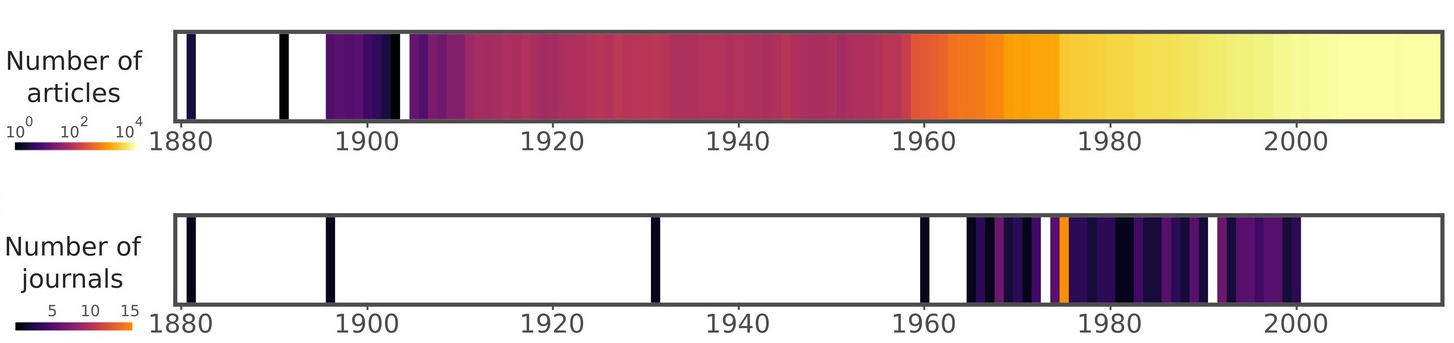
\includegraphics[width=400pt]{images/articles_up.png}
  \caption{Articles and Journals from 1880 to 2017. \parencite[]{read_down}}
  \label{fig:stdlift}
\end{figure}
\begin{figure}[h!]
  \centering
  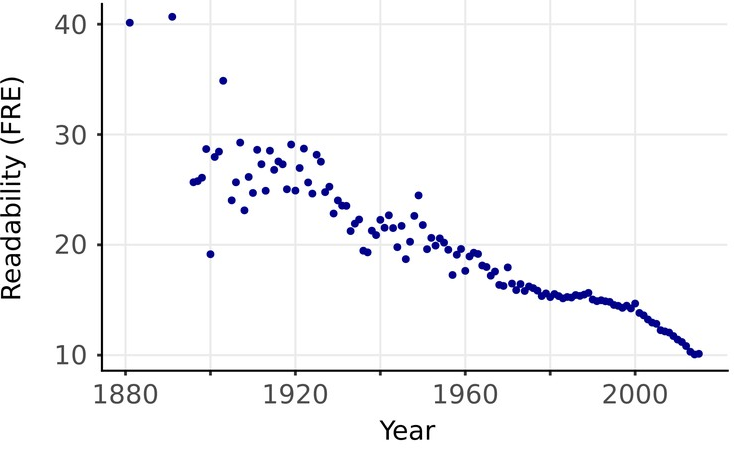
\includegraphics[width=400pt]{images/read_down.png}
  \caption{Mean Flesch Reading Ease (FRE) readability for each year. \parencite[]{read_down}}
  \label{fig:stdlift}
\end{figure}
\par 
This type of trend may be dangerous to the availability of research papers to the general public and even to inter field research. The less we can understand one another the less progress we make. Although the advancement of technology over the years may suggest that there is no need to fix this readability problem, we can also assume we have simply not hit the point where we can no longer understand ourselves with ease.
\par
Readability being such an important attribute for a well-written paper in any field makes study with Deep Learning practices more enticing. Passing a paper through machine eyes to quantify readability will prove a useful asset for future development.


\section*{Goal and Objectives}
 We seek to develop an application that can produce an accurate readability score for a Computer Science research paper. Taking traditional DL and ML methods and implementing a usable application to quantify readability.

\section*{Data and Methods}
In this research we will create a novel dataset from the Scopus database, the largest repository of scientific publications. We will collect all the publications available in the fields of Machine Learning till now from the database. A big chunk of time will be spent in generating and cleansing this data. We found approximately 300k publications in the database. We are downloading and cleaning this in a group of less than 2k papers because of the limitation set by the SCOPUS database. Then we will use traditional reading scoring algorithms to quantify those abstracts. After that, we will use the dataset and newly acquired score, to train a deep learning model. First, we are building a pre-model for testing purposes, with around 10k papers data, and measuring the accuracy with testing data.

\section*{Timeline}

\scalebox{1}{
\begin{tabular}{r |@{\timeline} l}

OCT Week-1 & Understanding Our Goals and Objectives with Project\\
\\
OCT Week-1 & Begin Data Gathering from SCOPUS\\
\\
OCT Week-1 & Work on Building Initial Model for Readability Analysis\\
\\
OCT Week-2 & Finding the Accuracy of our Predictions\\
\\
OCT Week 3 & Add more Data and Build Expanded Model\\
\\
OCT Week 4 & Use Model to Test Single Paper for Readability\\
\\
NOV Week 1 & Build Mock Production Interface for App\\
\\
3 Weeks Before Submission & Final Presentation\\
\\
 Last week of FALL'21 &  Complete Project Report Submission\\

\end{tabular}
}

\pagebreak

\printbibliography



\end{document}